\documentclass[a4paper,fleqn,usenatbib]{mnras}
\usepackage{newtxtext,newtxmath}
\usepackage[T1]{fontenc}
\usepackage{ae,aecompl}
\usepackage{graphicx}	% Including figure files
\usepackage{amsmath}	% Advanced maths commands
\usepackage{amssymb}	% Extra maths symbols
\usepackage{hyperref}

\def\grs{{GRS\,1739-278\,}}
\def\swiftx{{\em Swift-XRT\,}}
\def\swiftb{{\em Swift-BAT\,}}
\def\xmm{{\em XMM-Newton\,}}
\def\nustar{{\em NuSTAR\,}}
\def\integral{{\em INTEGRAL\,}}

\def\ferg{erg~cm$^{-2}$~s$^{-1}$}
\def\arcsec{''}
\def\degr{$^\circ$}
\def\arcmin{'}
\def\iaucirc{{IAU~Circ.}}

\title[Study of low-frequency QPO in \grs]{Study of low-frequency quasi-periodic oscillations in \grs during 2014 outburst}

%\author[I. A. Mereminskiy et al.]{
%Ilya A. Mereminskiy,$^{1}$\thanks{E-mail: i.a.mereminskiy@gmail.com}
%Andrey N. Semena,$^{1}$
%Sergey Bykov,$^{1,2}$
%Ekaterina V. Filippova$^{1}$
%\\
% List of institutions
%$^{1}$Space Research Institute, Russian Academy of Sciences, Profsoyuznaya 84/32, 117997 Moscow, Russia\\
%$^{2}$MGTU, Moscow, Russia\\
%}

\author[Authors]{
Authors$^{1}$
\\
% List of institutions
$^{1}$Space Research Institute, Russian Academy of Sciences, Profsoyuznaya 84/32, 117997 Moscow, Russia\\
%$^{2}$MGTU, Moscow, Russia\\
}


\date{Accepted XXX. Received YYY; in original form ZZZ}

\pubyear{2017}

\begin{document}
\label{firstpage}
\pagerange{\pageref{firstpage}--\pageref{lastpage}}
\maketitle

\begin{abstract}
\end{abstract}
We detected low-frequency quasi-periodic oscillations (QPOs) at 0.3..2 Hz in \nustar and \swiftx observations of black hole candidate \grs during its 2014 outburst.

\begin{keywords}
X-rays: individual (\grs)  -- accretion, accretion disks	
\end{keywords}


\section{Introduction}
\label{sec:intro} 


\section{GRS 1739-278}

\grs is a typical X-ray nova, discoveried during outburst in 1996  \citep{paul96} by SIGMA \citep{paul91} telescope onboard GRANAT space observatory. During this outburst \grs demonstrated
Using {\it ROSAT} observation \cite{greiner96} inferred distance of 6--8.5~kpc, indicating that source may belong to Galactic bulge.	
%\grs was discovered in 1996 by SIGMA telescope onboard GRANAT space observatory  \citep{paul96}.  
%Later GRANAT continued observations of this source \citep{vargas97} along with other X-ray telescopes: ROSAT \citep{greiner96}, RXTE and TTM/Kvant \citep{borozdin98}. The optical counterpart was found in observations carried out by ESO telescopes \citep{marti97}. . During the outburst \grs demonstrated typical behavior of the black hole candidate \citep[BHC, see e.g.][]{grebenev93, grebenev97, tanaka96, remillard06, belloni10}. The lightcurve could be described with a FRED-like (fast rise, exponential decay) shape, at the beginning of the outburst the source was in a typical low/hard state, with spectrum dominated by a power-law component with exponential cutoff at high ($\ge$100 keV) energies followed by a high/soft state with a strong blackbody component \citep{borozdin98}. Observations at VLA \citep{durouchoux96} revealed presence of variable radio emission, which could be caused by jets.  \cite{borozdin00} found QPO at 5 Hz in RXTE observations conducted while the source was in the very high/soft state.

%The onset of 2014 outburst was detected by \swiftb \citep{krimm14_atel} along with \integral \citep{filippova14}. 

%At the beginning of the September, 2016 there was another, third, outburst, that 

\begin{figure*}
\centerline{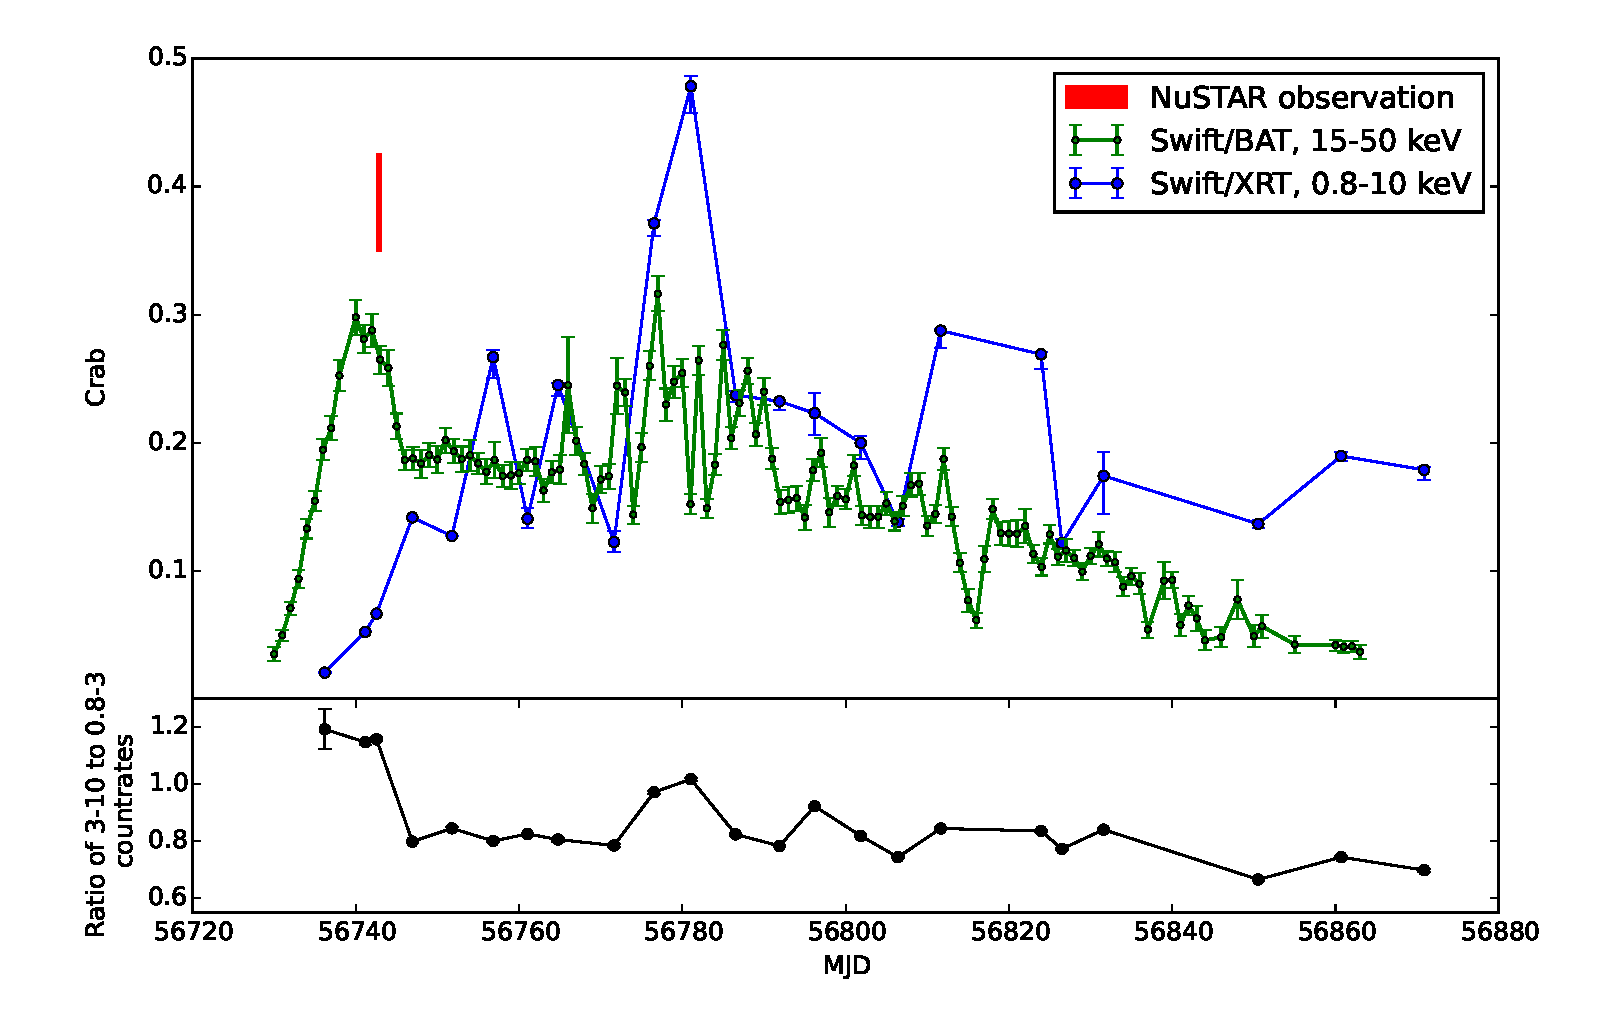
\includegraphics[scale=0.5]{batlc_v05.eps}}
\caption{{\it Upper:} green points denote \swiftb\, lightcurve of second outburst in 15--50 keV range, blue circles correspond to \swiftx\, fluxes in 0.8--10 keV. Red line show time of \nustar\, observation. {\it Lower:} evolution of \swiftx\, spectral hardness during the outburst.} 
\label{fig:batlc}
\end{figure*} 

\section{Observations and data reduction}
\label{sec:datared} 
We used public observations of \swiftx\, (target ID: 33203) performed regular over the peak and decline of the outburst.  Since the source was bright, all \swiftx\, observations were performed in windowed mode, allowing study of timing properties of the source. We performed standard analysis with {\texttt{xrtpipeline}} and barycentered data prior to lightcurve extraction.\\
We also used \nustar\, observation (ObsID: 80002018002) performed at March 26, 2014 (MJD 56742).  We used standard pipeline to extract all photons from two-arcminute circular region, centered on source. Lightcurves and spectra were produced through standart pipeline.



\section{Analysis}
\subsection{Outburst}
First detection of the source by \swiftb\, \citep{krimm14_atel} occured at March 9, 2014 (MJD 56725, we will refer to this date as $\tau_{0}$), onset of outburst was the confirmed by \integral \citep{filippova14}. Outburst profile in hard X-rays (15--50~keV) featured fast rise with tenfold intensity increase over ten days, nearly flat-top peak ($\tau_{0}$+10..+15) followed by abrupt flux decrease by 30\% over two days. After this, source demonstrated gradual decline interrupted by flaring activity at $\tau_{0}$+30..+65. Another interesting feature is dip, observed in \swiftb lightcurve at $\tau_{0} \approx 86$. After the cease of the outburst source remained active with flux about 5--15 mCrab. 

Adding \swiftx\, data to the \swiftb\, gives us another insight on evolution of the outburst as shown in Fig.\,\ref{fig:batlc} - comparing fluxes in soft and hard bands (for 0.8--10 keV band we took a 3000 counts s$^{-1}$ as a reference value for Crab, corresponding value for 15--50 keV band is 0.22 cts cm$^{-2}$ s$^{-1}$) one can see that soft component obviously lags hard emission in the beginning of the outburst but then start to grow and ends up dominating during the flaring period as well as hard dip. This type of behavior is typical for black hole candidates \citep[BHC, see e.g.][]{grebenev97, tanaka96, remillard06, belloni10} - outburst starts from low-hard state, then proceeds to the high-soft (or even very-high-soft state, as were seen in 1996 outburst \citep{borozdin00}) and then returns back to low-hard state and, eventually, to quiescence. Lower subplot of Fig.\,\ref{fig:batlc} shows evolution of hardness ratio (3--10~keV/0.8--3~keV) measured by \swiftx. Right after peak of hard X-rays one can see decline of hardness, indicating appearance of thermal component.

Fortunately, the \nustar\, \citep{harrison13_nust} observation triggered by \cite{miller15_nust} were carried right at the transition between hard and soft states, thus giving us unique possibility to study processes that happens during transition. 

\subsection{NuSTAR observation}
\label{sec:nust} 

\nustar\, observed \grs (ObsID: 80002018002) for nearly 30 ks of dead-time corrected exposure right after hard X-ray peak (see Fig.~\ref{fig:batlc}). Earlier, \cite{miller15_nust} shown that the average spectrum of this observation is well described by reflection models such as {\it relxill} \citep{dauser14,dauser16} with accretion disk that reaches remarkably close to the black hole innermost stable circular orbit (ISCO), with upper estimate being $r_{in} = 5^{+3}_{-4}\, G M/c^{2}$. 
Interestingly, no additional thermal component was needed in order to obtain a good fit, probably because of \nustar\, energy band, starting at 3~keV. 

Given the 96.9 minute orbital period of \nustar, observation is divided in 13 intervals separated by Earth occultations, as shown in Fig.\,\ref{fig:nust_lc}. We denoted this intervals with roman numerals, from {\bf I} to {\bf XIII}. From the lightcurve of observation it is clear, that source flux is increasing throughout observation from $\approx$145 counts per second up to $\approx$170 counts per second. 
The spectrum also alter, with hardness (defined as ratio of countrates  $R_{3-10\,keV}/R_{10-78\,keV}$) monotonically growing from 2.5 to 3.5. 
Since it is obvious that the source spectrum is somehow changing during the observation it is interesting to check if Fe-line profile stays the same during observation or changes. 
We split observation into three major pieces, with first made by intervals {\bf I-IV}, second by {\bf V-IX} and third by {\bf X-XIII} and extracted 3--78 keV spectra. 
We chose to group them in order to have at least 100 counts per bin. 
Then we fitted them (excluding data below 4 keV and between 5--10 keV) with simple \texttt{phabs*cutoffpl} model, using $N_{H} = 2.15\times10^{22}$ cm$^{-2}$ as was found by joint \xmm/\nustar\, observation during low luminosity state \citep{fuerst16}. 
Now, plotting the ratio of this fit to initial spectra (see Fig.~\ref{fig:ratios}) one can see that both strong features - i.e. Fe-line complex at 5--9 keV and Compton hump around 30 keV are seemingly stable. 
Parameters of the cut-off powerlaw change slightly from part to part: photon index grows from 1.48 to 1.52 and then to 1.56 , while energy of exponential rollover changes from 28.5 keV to 27.8 keV and then to 27.4 keV. 

\begin{figure*}
\centerline{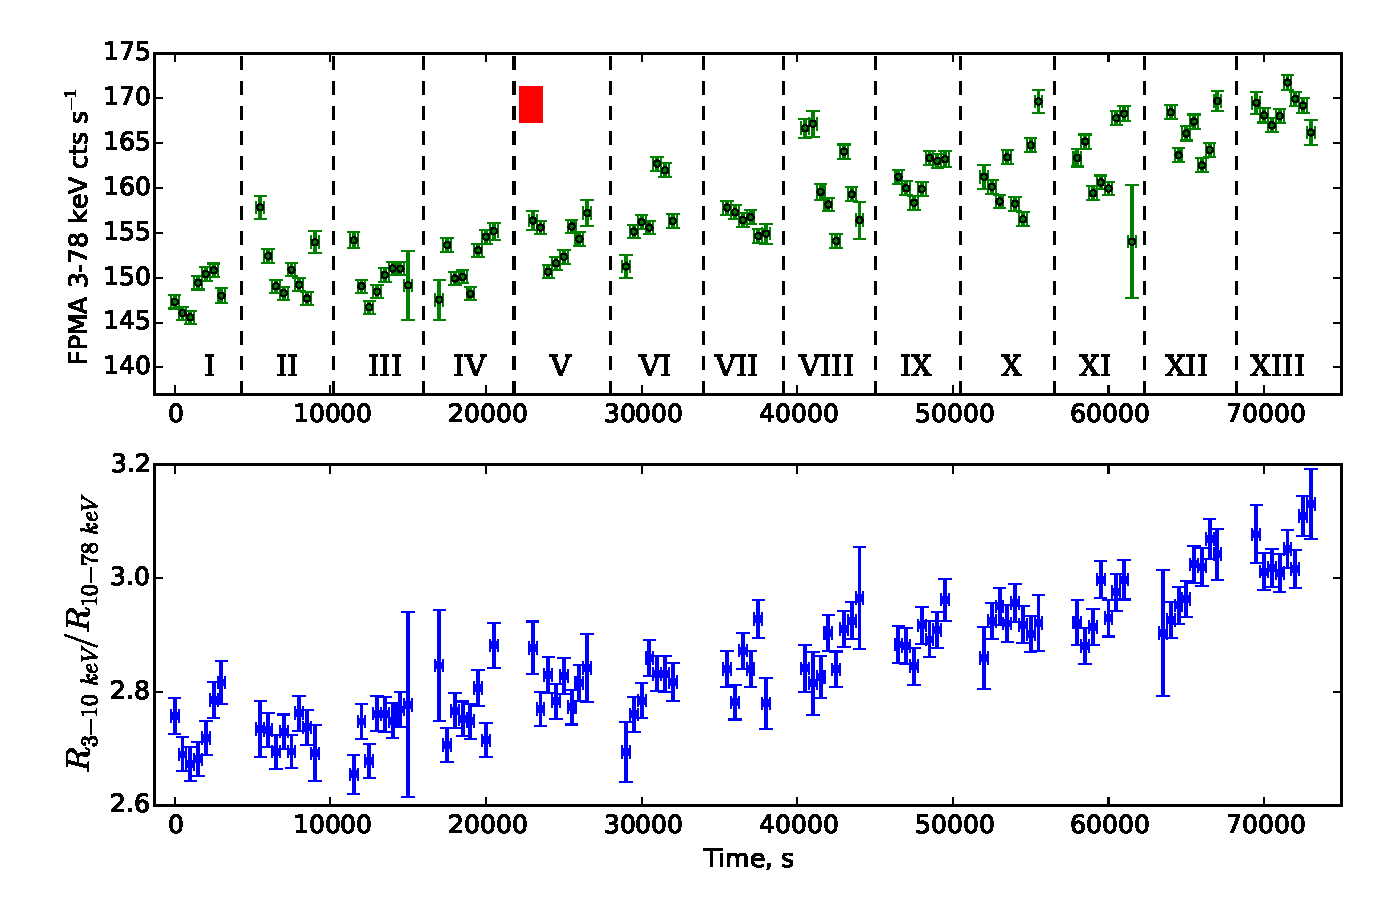
\includegraphics[scale=0.7]{nuAlc_color_v04.eps}}
\caption{Upper panel: countrate of \nustar\,FPMA in 3--78 keV band. We enumerated intervals of uninterrupted observations with roman numerals. Red square shows time of simultaneous \swiftx observation (ObsId: 00033203003, second part). Bottom panel: evolution of hardness during observation} 
\label{fig:nust_lc}
\end{figure*} 

 \begin{figure}
\centerline{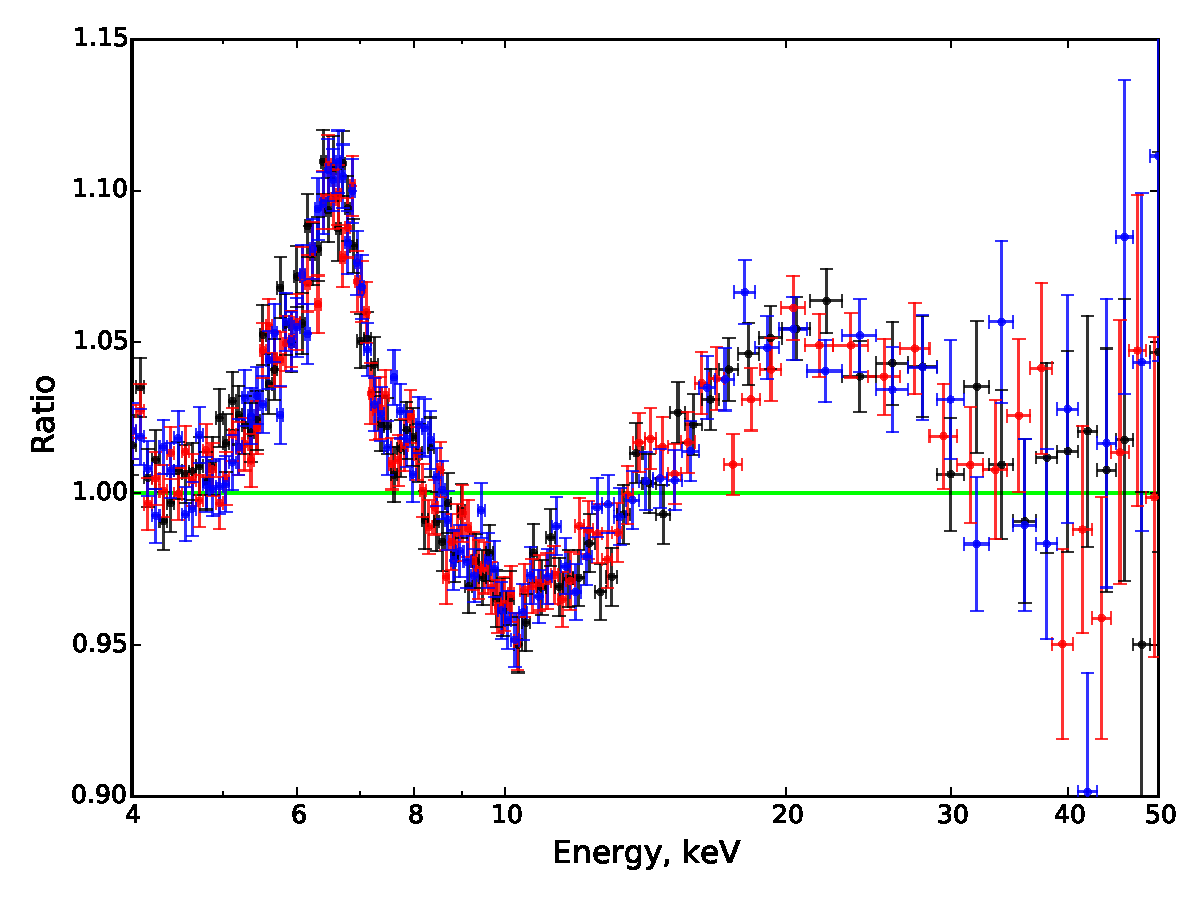
\includegraphics[width=\linewidth]{ratios_v01.pdf}}
\caption{Ratio of \nustar\, spectra to \texttt{phabs*cutoffpl} model. In black - data from intervals I-IV, in red from V-IX and in blue from X-XIII.} 
\label{fig:ratios}
\end{figure}  
            
From visual inspection of Fig.~\ref{fig:ratios} it is seen that nor line profile, nor Compton hump did not changing significantly between parts of the observation.


There is a 1 ks part of \swiftx\, observation, that coincides with ??? of \nustar\, observation, we decided to treat that data simultaneously, thus covering energies from 0.8 to 78 keV. 
We used latest availiable version of {\it relxill} package (v1.0.2). 
Element abundances were taken from \cite{wilms00} and cross-sections from \cite{verner96}.

\begin{figure*}
\centerline{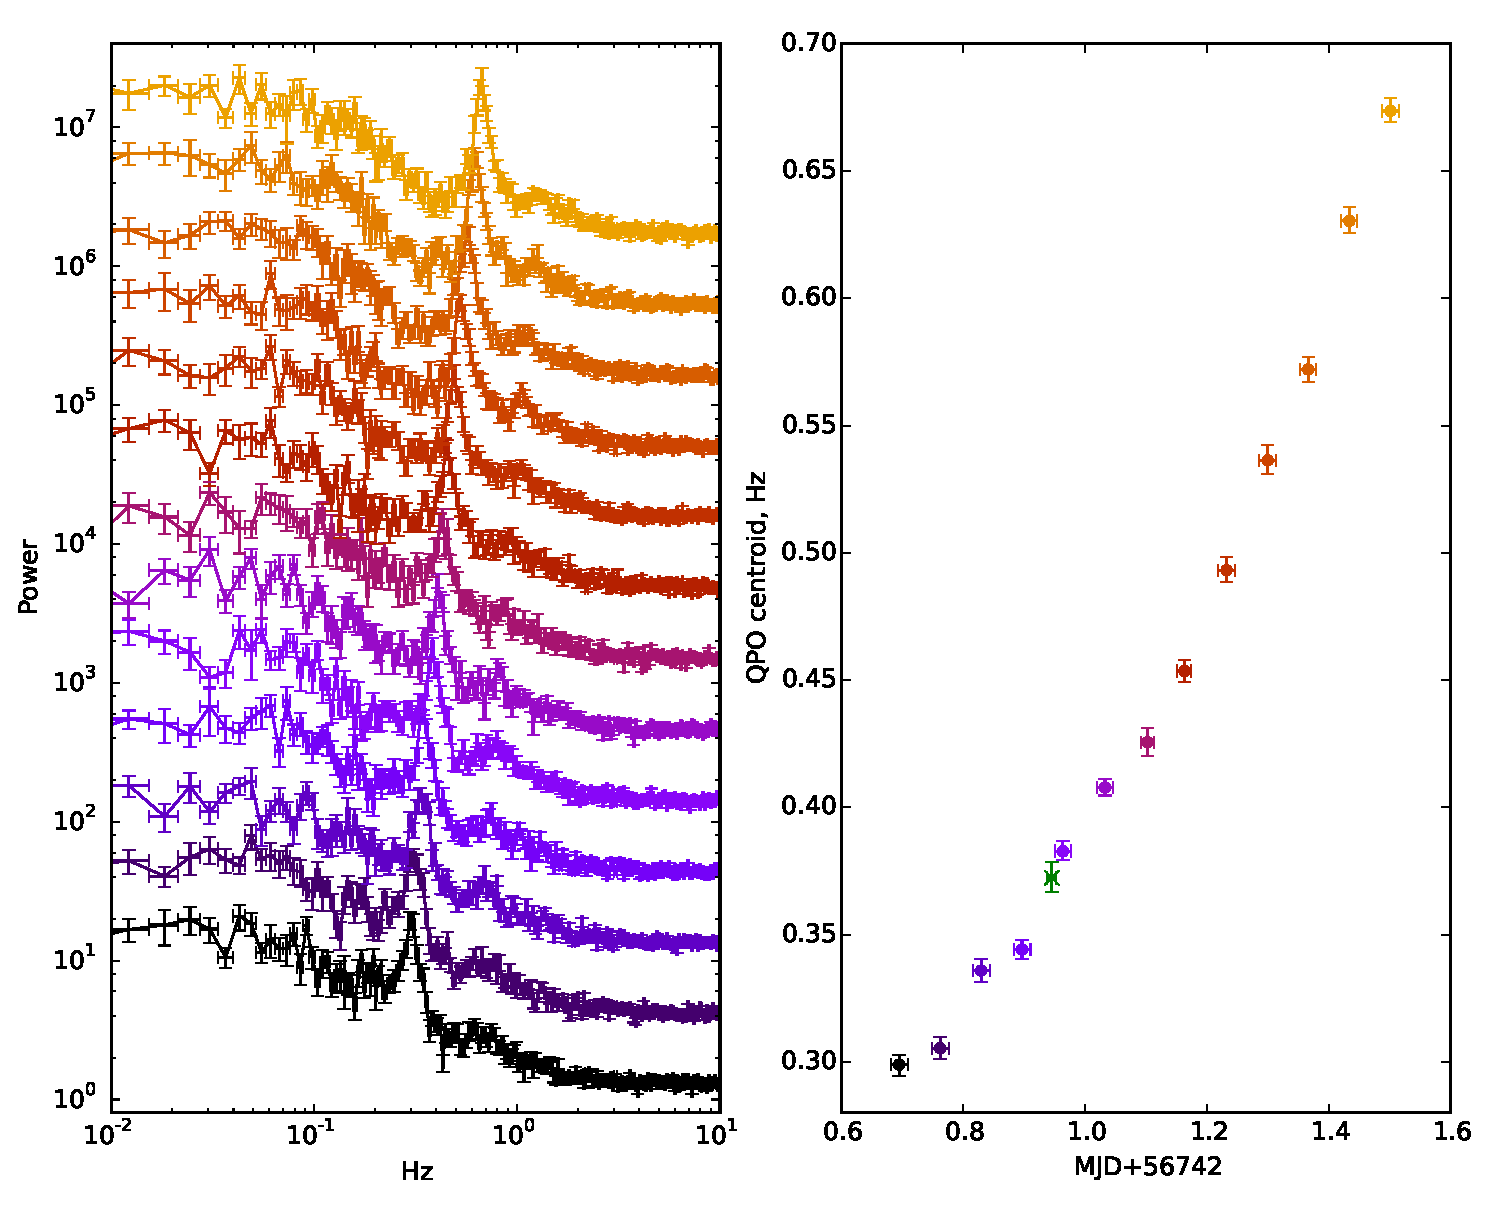
\includegraphics[scale=0.7]{QPOdrift_v02.eps}}
\caption{Change of the QPO frequency with time. On the left panel we show how power-density spectra change with time - for clarity each spectrum is multiplied by a factor of 3.25. On the right panel we show how the QPO frequency changes during observation. Green cross show QPO frequency derived from \swiftx\, observation.} 
\label{fig:qpodrift}
\end{figure*}  


\section*{Acknowledgments}

%--------------------------------------------------------------------------------
\bibliographystyle{astron}
\bibliography{author_en.bib}
\bsp	
\label{lastpage}
\end{document}
